\documentclass[a4paper]{article}

\usepackage[english]{babel}
\usepackage{microtype}
\usepackage{graphicx}
\usepackage{amsmath}
\usepackage{index}
\usepackage{mathtools}

\makeindex

\begin{document}
	\title{\large{\textbf{Compte rendu TP3}}\\ Robot Khepera}
	\author{Arthur VAIN, Valentin Dosias, Maxence NEUS}
	\date{}
	
	\maketitle	
	\tableofcontents
	\newpage
	
	\section{Introduction}
	L'objectif de ce TP est l'étude des différentes actions d'un régulateur PID à travers 2 commandes différentes: la commande en position et la commande en vitesse.
	
	Le robot étudié sera un robot mobile de type Khepera II possédant 2 roues motrices pilotés par des moteurs à courant continu grâce auxquels nous commanderons celui-ci.
	Pour ce faire, nous communiquerons avec ce robot via une liaison série en utilisant Matlab.
	
	\section{Etude préliminaire}
	Nous allons utiliser le système d'équation de mouvement décrit dans le sujet :
	$$
	\begin{cases}
		F_{x1} + F_{x2} = m.\ddot{x}\\
		(F_{x1} - F_{x2}).\dfrac{d}{2} = I_{z}.\ddot{\alpha}\\
		U_{1} = J_{1}.\ddot{\theta}_{1} + f_{1}.\ddot{\theta}_{1} + F_{x1}.R\\
		U_{2} = J_{2}.\ddot{\theta}_{2} + f_{2}.\ddot{\theta}_{2} + F_{x2}.R\\
	\end{cases}
	$$
	On utilise ce système d'équations pour déterminer les égalités matricielles suivantes :
	\begin{equation}
	\begin{bmatrix}
	\ddot{x} \\
	\ddot{\alpha} \\
	\ddot{\theta}_{1} \\
	\ddot{\theta}_{2} \\
	\end{bmatrix}
	=
	\begin{bmatrix}
	0 & 0 & 0 & 0 \\
	0 & 0 & 0 & 0 \\
	0 & 0 & -\dfrac{f}{J} & 0 \\
	0 & 0 & 0 & -\dfrac{f}{J} \\
	\end{bmatrix}
	\begin{bmatrix}
	\dot{x} \\
	\dot{\alpha} \\
	\dot{\theta}_{1} \\
	\dot{\theta}_{2}
	\end{bmatrix}
	+
	\begin{bmatrix}
	\dfrac{1}{m} & \dfrac{1}{m} & 0 & 0 \\
	\dfrac{d}{2.I} & -\dfrac{d}{2.I} & 0 & 0 \\
	-\dfrac{R}{J} & 0 & \dfrac{1}{J} & 0 \\
	0 & \dfrac{R}{J} & 0 & \dfrac{1}{J} \\
	\end{bmatrix}
	\begin{bmatrix}
	F_{1} \\
	F_{2} \\
	U_{1} \\
	U_{2} \\
	\end{bmatrix}
	\end{equation}
	On note également l'égalité :
	\begin{equation}
	\begin{bmatrix}
	\dot{\theta}_{1} \\
	\dot{\theta}_{2} \\
	\end{bmatrix}
	=
	\begin{bmatrix}
	0 & 0 & 1 & 0 \\
	0 & 0 & 0 & 1 \\
	\end{bmatrix}
	\begin{bmatrix}
	\dot{x} \\
	\dot{\alpha} \\
	\dot{\theta}_{1} \\
	\dot{\theta}_{2}
	\end{bmatrix}
	+ 
	\begin{bmatrix}
	0 & 0 & 0 & 0 \\
	0 & 0 & 0 & 0 \\
	\end{bmatrix}
	\begin{bmatrix}
	F_{1} \\
	F_{2} \\
	U_{1} \\
	U_{2} \\
	\end{bmatrix}
	\end{equation}
	Ces deux équations matricielles nous permettent d'utiliser le bloc "state space" de simulink pour obtenir les valeurs de $\dot{\theta}_{1}$ et $\dot{\theta}_{2}$. \\
	
	Nous utilisons ensuite le systèm d'équation suivant pour déterminer les vitesses du robot à partir de $\dot{\theta}_{1}$ et $\dot{\theta}_{2}$.
	$$
	\begin{cases}
	\dot{u} = \dfrac{\dot{\theta}_{1}+\dot{\theta}_{2}}{2}.R;\\
	\dot{\alpha} = \dfrac{\dot{\theta}_{1}-\dot{\theta}_{2}}{d}.R;\\
	\dot{v} = \dfrac{\dot{\theta}_{1}-\dot{\theta}_{2}}{d}.R.r_{1}\\
	\end{cases}
	$$
	\newpage
	Nous projetons ensuite dans le repère global affin d'obtenir la position du robot.
	On obtient alors le schéma bloc suivant :
	\begin{figure}[h]
		\centering
		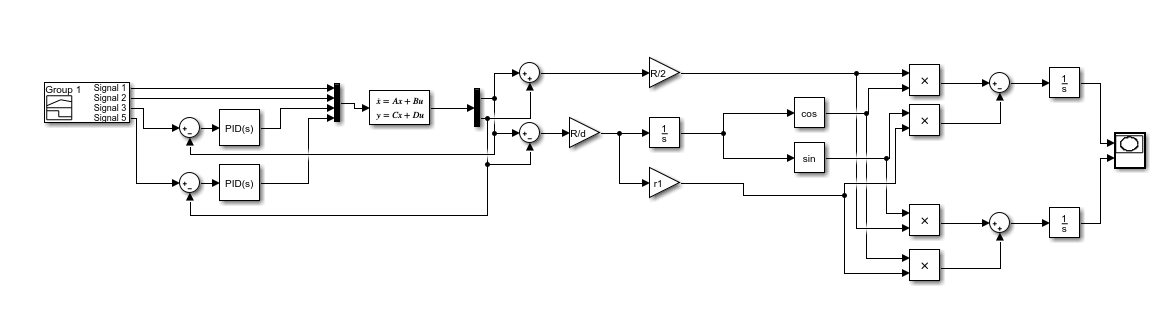
\includegraphics[width = 13cm]{Khepera.png}
		\caption{Schéma bloc du robot}
	\end{figure}
	\\
	On notera que les caractèristiques $\dot{\theta}_{1}$ et $\dot{\theta}_{2}$ sont commandées par deux régulateur PID (on les supposera identiques) qui sont ceux que l'on va étudier dans la partie qui suit.
	
	\section{Etude experimentale}
	\subsection{PID pour la commande en position}
		Tout d’abord, nous avons commencé par commander le robot en position.
		Nous avons essayé de mettre une valeur faible de P (1-2-5) mais rien ne se passait lorsqu’il n’y avait pas d’autre composante dans le régulateur. Nous avons donc testé avec P=5 D=0 et I=1, nous avons obtenu un temps de réponse à 5\% d’environ 3.4 s avec un léger dépassement mais aucune erreur statique lorsque le régime devient stable.
		Nous avons augmenté la valeur de P à 20, on gagne environ 0.1 sec sur le temps de réponse et le temps où l'erreur est présente est plus court.
		
		
		\begin{figure}[h]
			\centering
			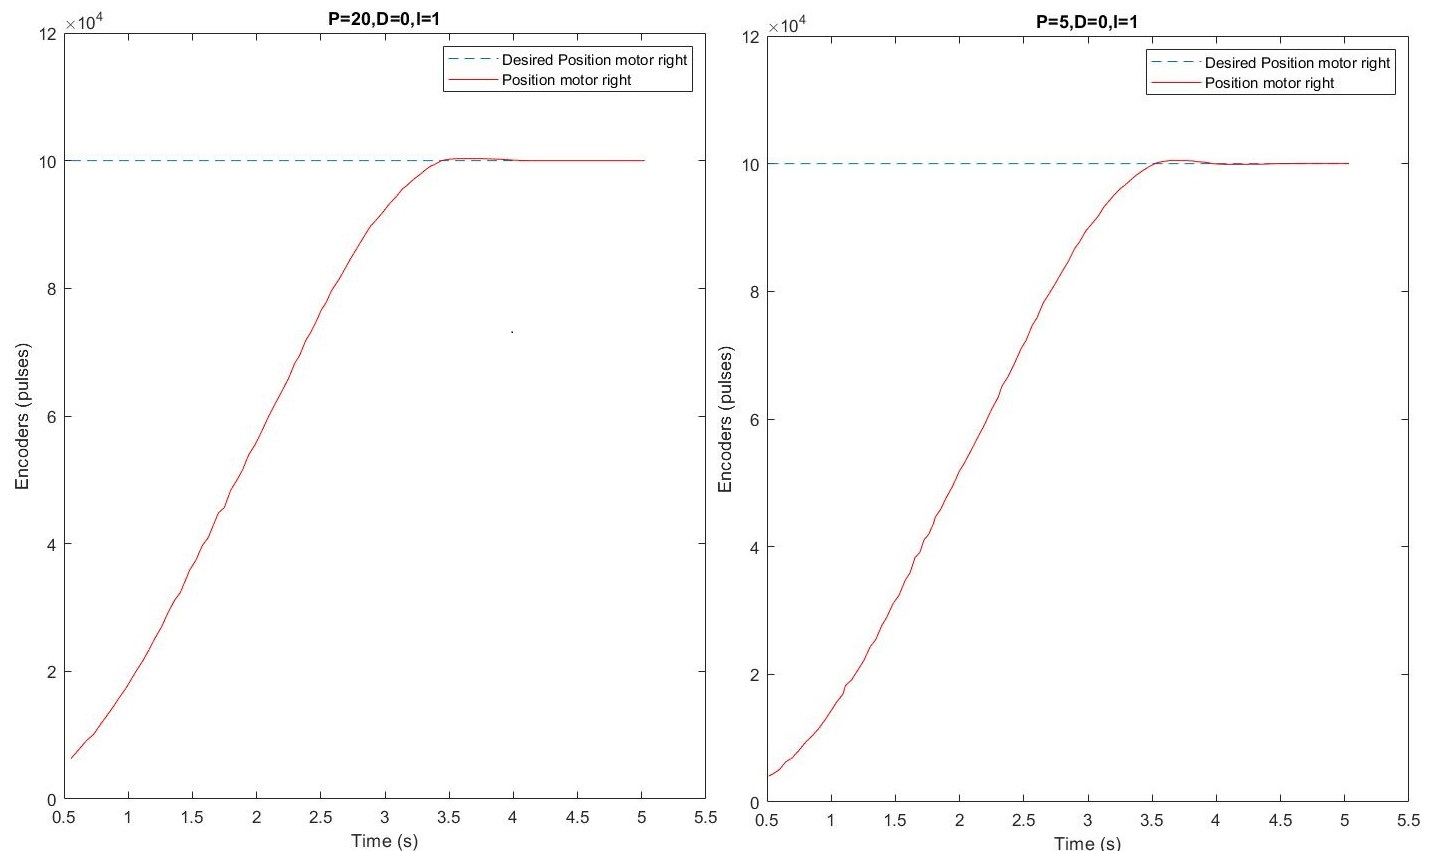
\includegraphics[width = 9cm]{imgs/fig1.jpg}
			\caption{Comparaison entre une action proportionnelle à 5 et 20}
		\end{figure}
		Pour voir vraiment l’effet de l’action proportionnelle nous avons enlever l’action intégrale sans laquelle le robot ne marchait pas pour une valeur de P assez faible.
		Nous obtenons une erreur beaucoup plus importante et longue sans pour autant que le temps de réponse ne change beaucoup. Nous essayons de corriger l’erreur avec un intégrateur faible (I=1, D=0). Dans ce cas le système n’est plus stable, l’erreur est trop importante. Nous pouvons donc en conclure que pour le robot l’écart entre les différentes actions ne doit pas être trop élevé.
		
		\begin{figure}[h]
			\centering
			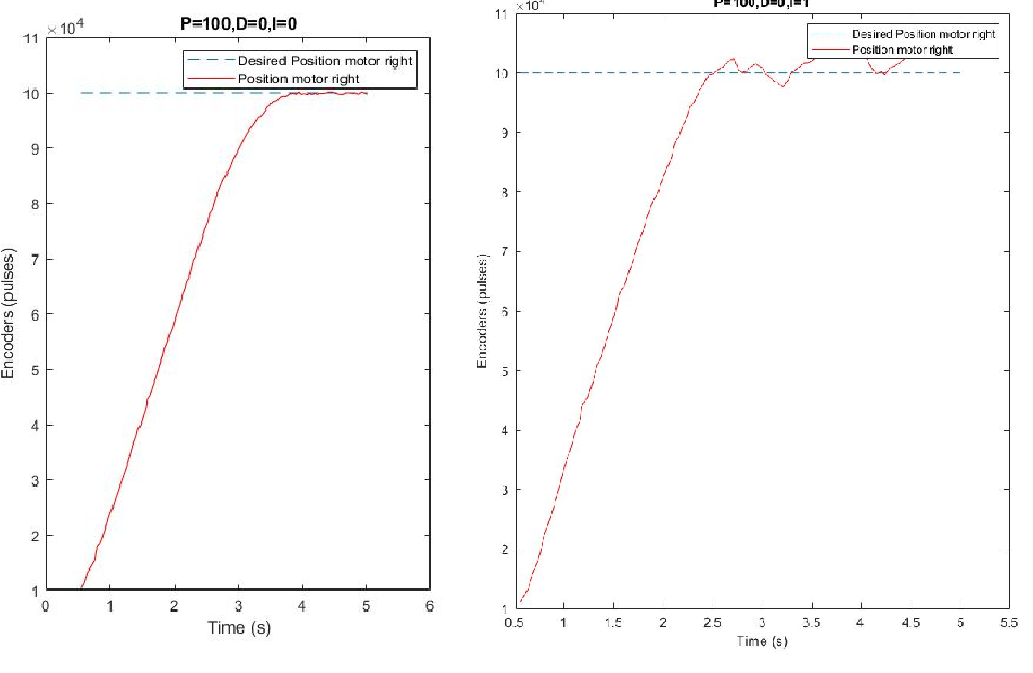
\includegraphics[width = 9cm]{imgs/fig2.png}
			\caption{}
		\end{figure}
		Nous avons encore augmenté l’intégrateur (I=10) en diminuant la consigne. Le système oscillait et ne devenait jamais stable. Nous avons ensuite changé l’action et mis P=50. Le système était stable avec une erreur qui oscillait toujours mais moins importante que dans les cas précédents. Cela confirme notre observation que pour le robot la proportionnalité entre les différentes actions doit être assez faible.
		
		\begin{figure}[h]
			\centering
			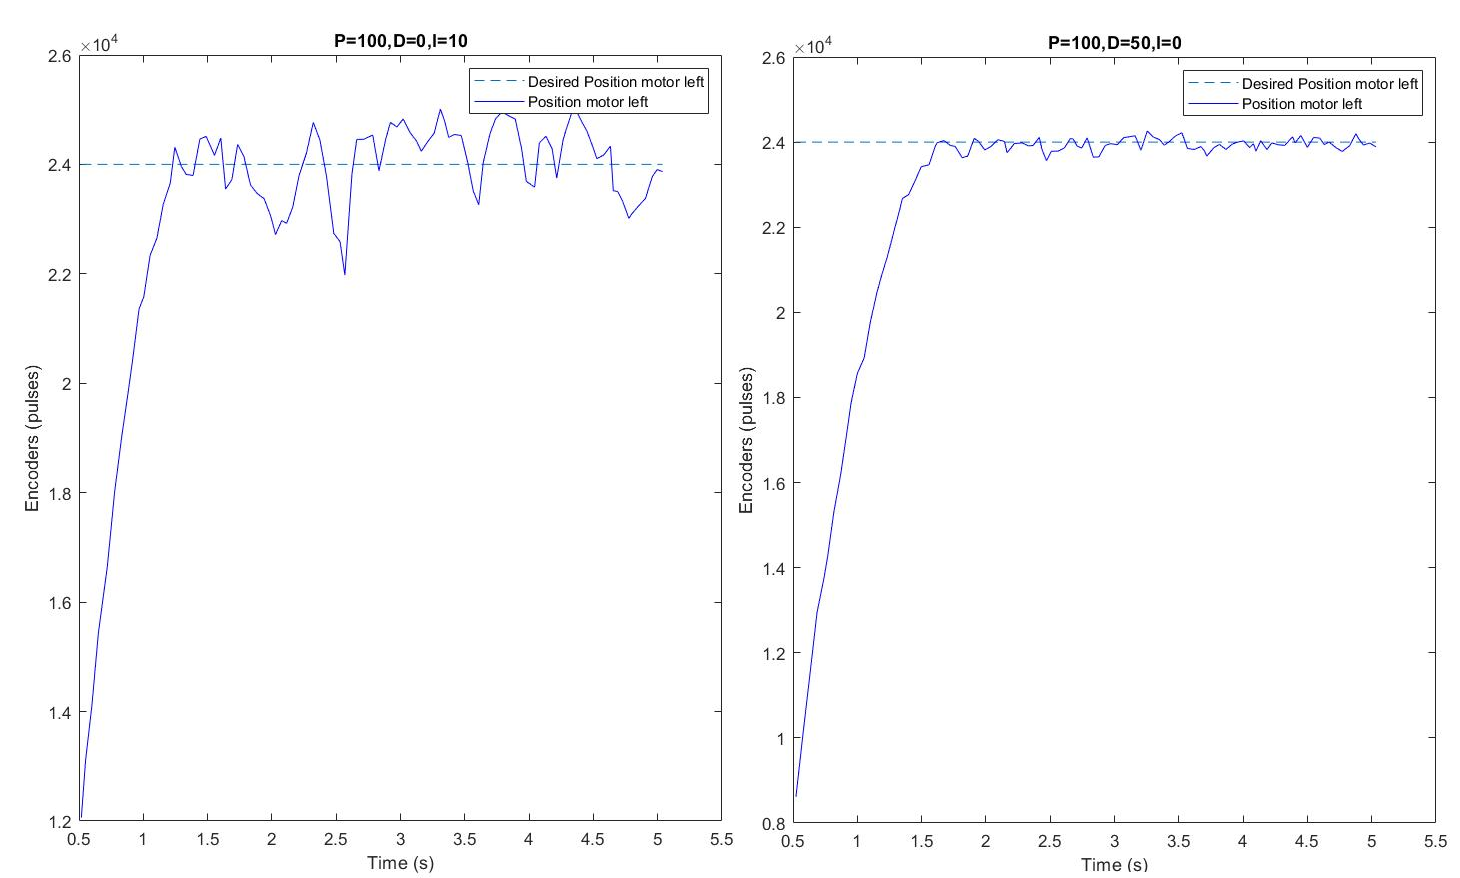
\includegraphics[width = 9cm]{imgs/fig3.png}
			\caption{}
		\end{figure}
		Nous avons diminué la valeur de l’action intégrale à 5 pour mieux voir son influence. Nous obtenons un temps de réponse plus faible (entre 3.1 et 3.2 secondes) sans dépassement ni erreur statique.
		Nous avons essayé de faire fonctionner le robot avec un régulateur P=5 et D=5 et I = 0, cette configuration n’a pas permis au robot de fonctionner. Nous avons ajouté un léger intégrateur (P=5 et D=5 et I = 1). Nous obtenons un temps de réponse de 5\% de 3.4 s avec un dépassement plus important que précédemment. Nous avons augmenté à 20 pour mieux voir son effet car nous ne pouvons rien conclure de l’essai précédent.  Le temps de réponse diminue légèrement 3.3 sec et le dépassement est légèrement plus important.
		
		\begin{figure}[h]
			\centering
			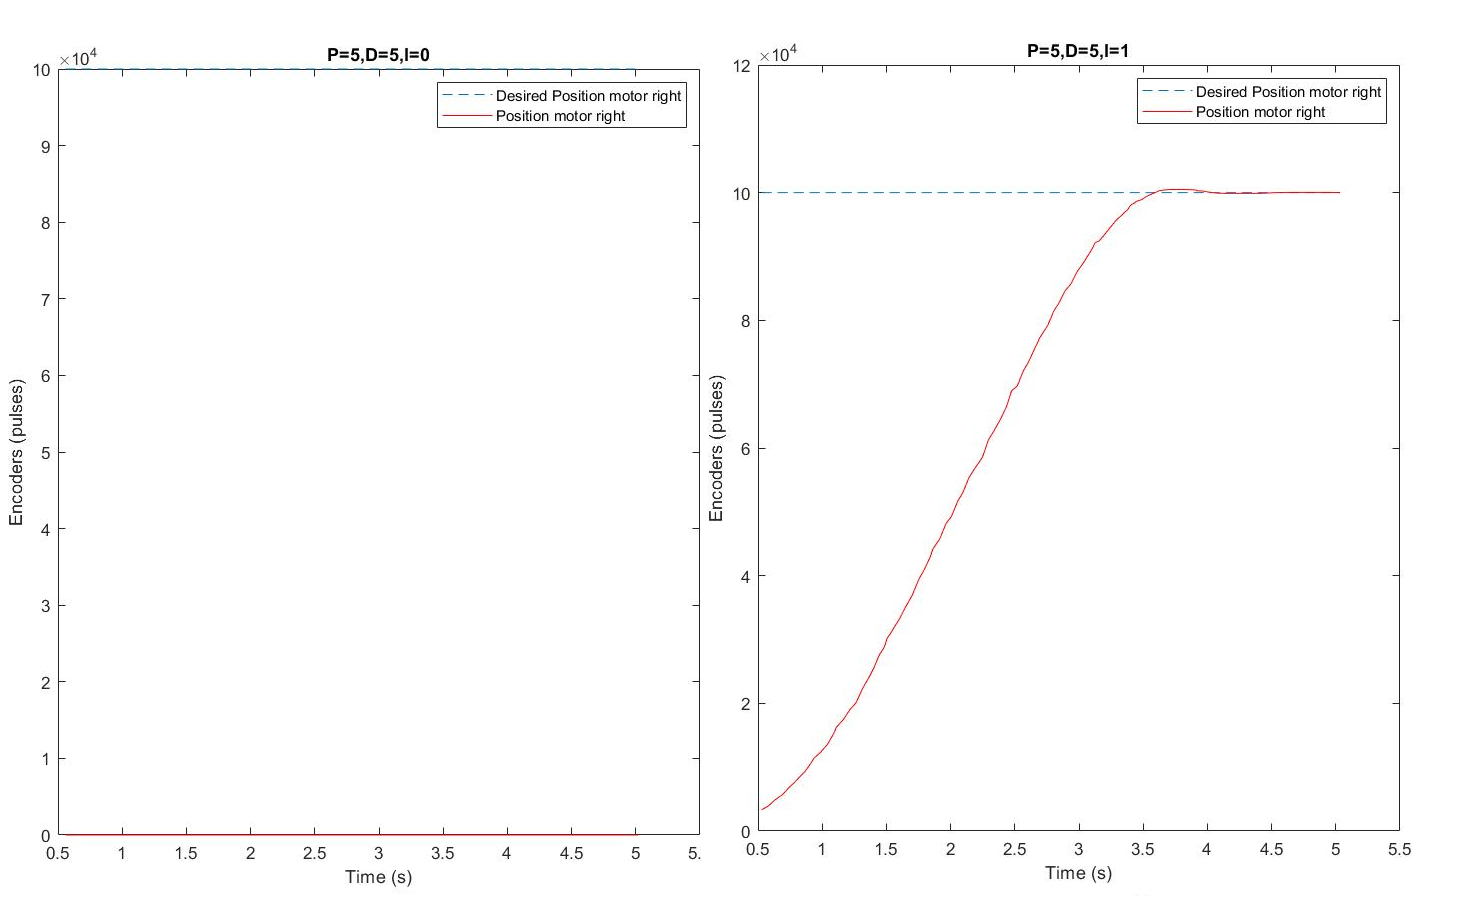
\includegraphics[width = 9cm]{imgs/fig4.png}
			\caption{}
		\end{figure}
		Pour finir nous avons testé, les réglages du programme par défaut soit P=5, D=5 et D=10.Nous avons un temps de réponse entre 3.1 et 3.2 ce qui est mieux qu’avec seulement 2 des 3 actions. Nous n’avons aucun dépassement ni aucune erreur. Nous voyons donc que quand les 3 actions sont bien réglées, les performances sont optimales.
		
		\begin{figure}[h]
			\centering
			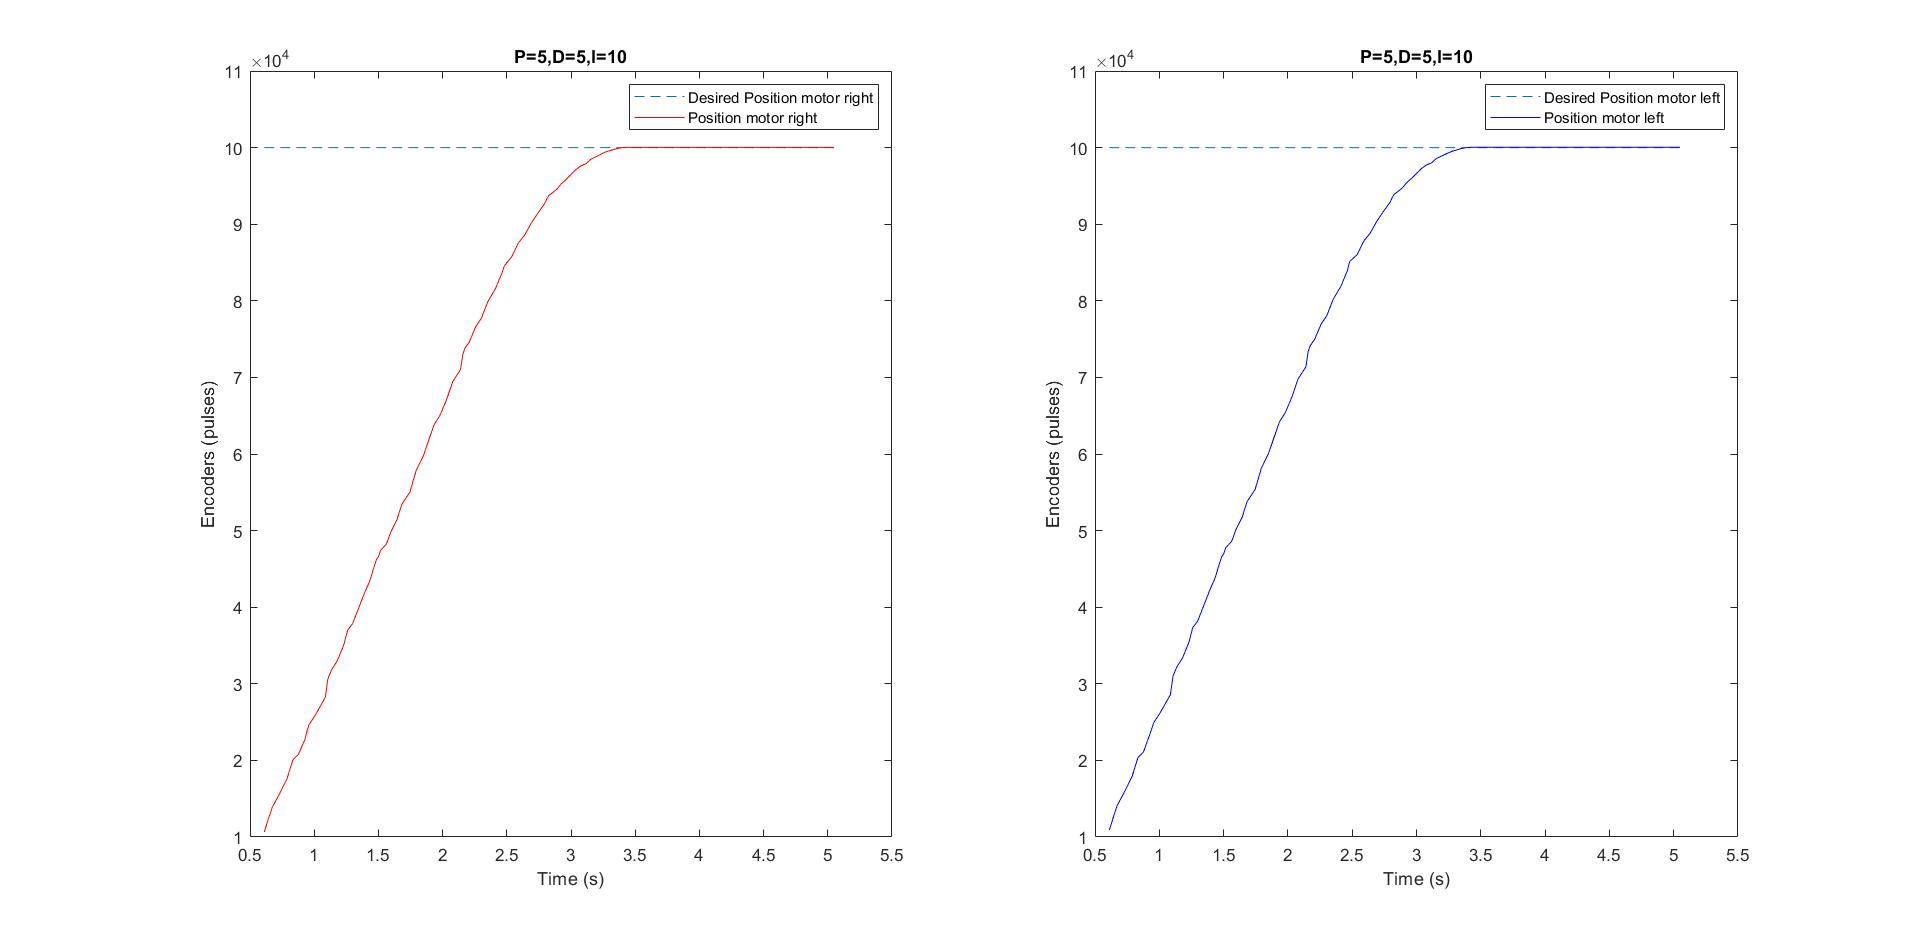
\includegraphics[width = 11cm]{imgs/fig5.jpg}
			\caption{}
		\end{figure}
		Après avoir mesuré avec une règle nous avons mesuré et déduit que le robot avance de 1 cm pour 1500 points 
		
	\subsection{PID pour la commande en vitesse}
	
		Nous avons d’abord essayé une action proportionnelle seule. La consigne était de 500. Le robot n’arrive qu'à 200 et quand l’action est à 40, le robot arrive à 370, nous ne voyons pas de temps de réponse pour arriver à cette valeur. Nous en déduisons que pour que le robot fonctionne correctement nous devons au moins avoir l’action proportionnelle et une des deux autres actions.
		Nous allons maintenant étudier l’effet des autres actions.
		Nous réglons maintenant à P=10 I=1 et D=0. Nous obtenons un temps de réponse d’environ 2.3 sec mais nous avons toujours une erreur variable, la consigne n’est pas strictement atteinte.
		Nous augmentons ensuite le I = 10, nous ne voyons plus le temps de monté mais la valeur 750 (consigne = 500) et atteinte à 0.6 sec, le dépassement est très important, le système met 1 seconde à être stable, c’est assez peu mais le dépassement est trop important et l’erreur n’est pas trop différente comparé à I=1.
		\begin{figure}[h]
			\centering
			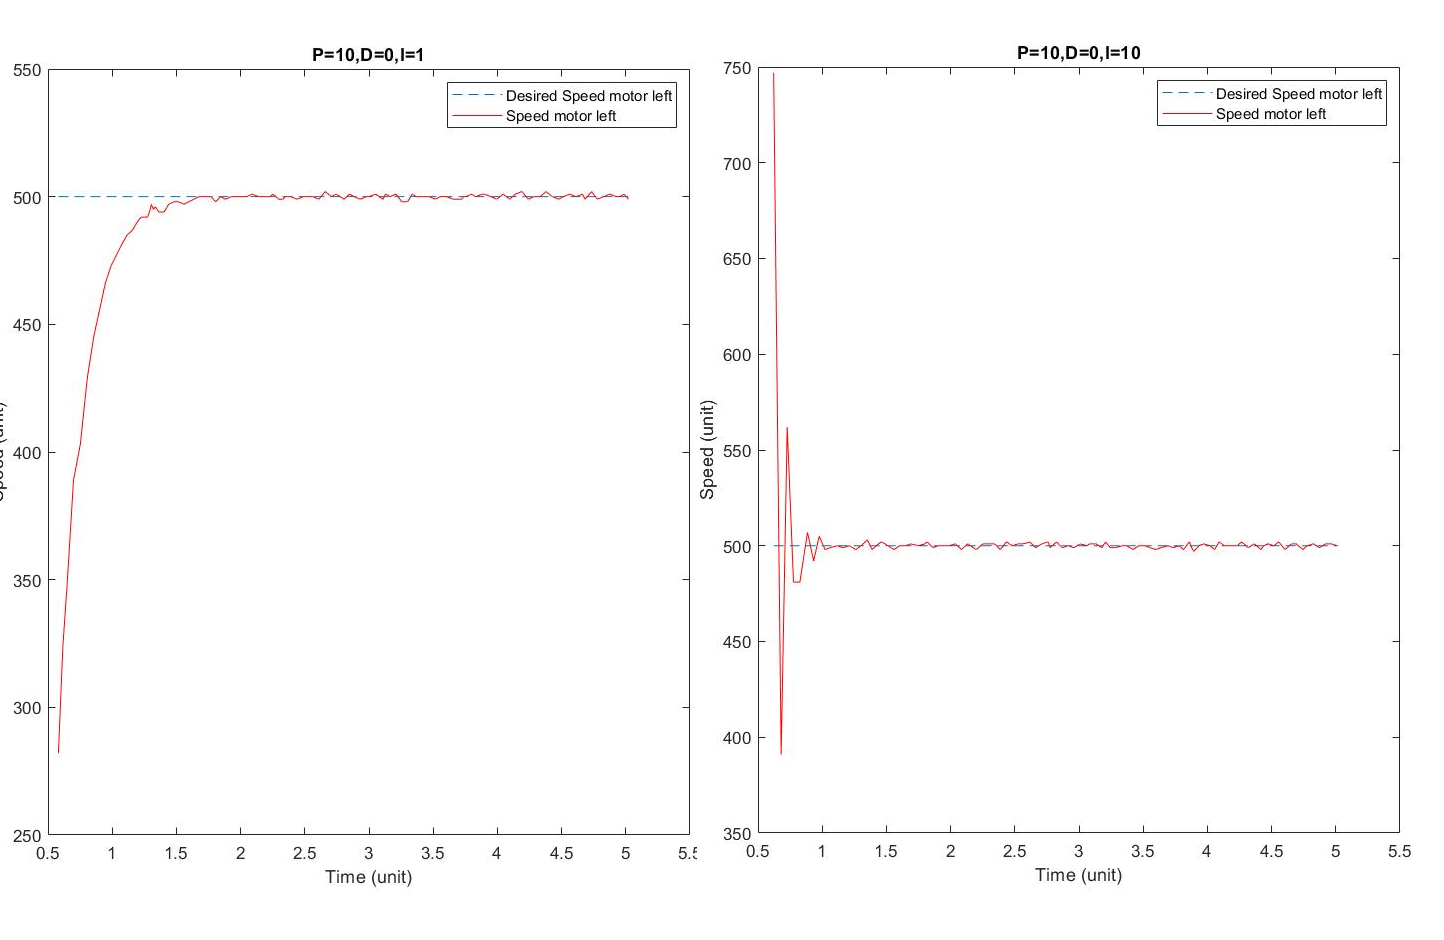
\includegraphics[width = 9cm]{imgs/fig6.png}
			\caption{}
		\end{figure}
		Nous pouvons conclure que d’augmenter autant l’action intégrale n’est pas bien pour le système.
		Nous allons maintenant étudier l’action dérivée. On règle à P=10, I=0 et D=1. Avec cette configuration, le système n’arrive pas à la consigne.  Le résultat est le même en augmentant l’action dérivée à 10. Pour le robot, il faut donc que les 3 composantes soient non nulles.
		
		\begin{figure}[h]
			\centering
			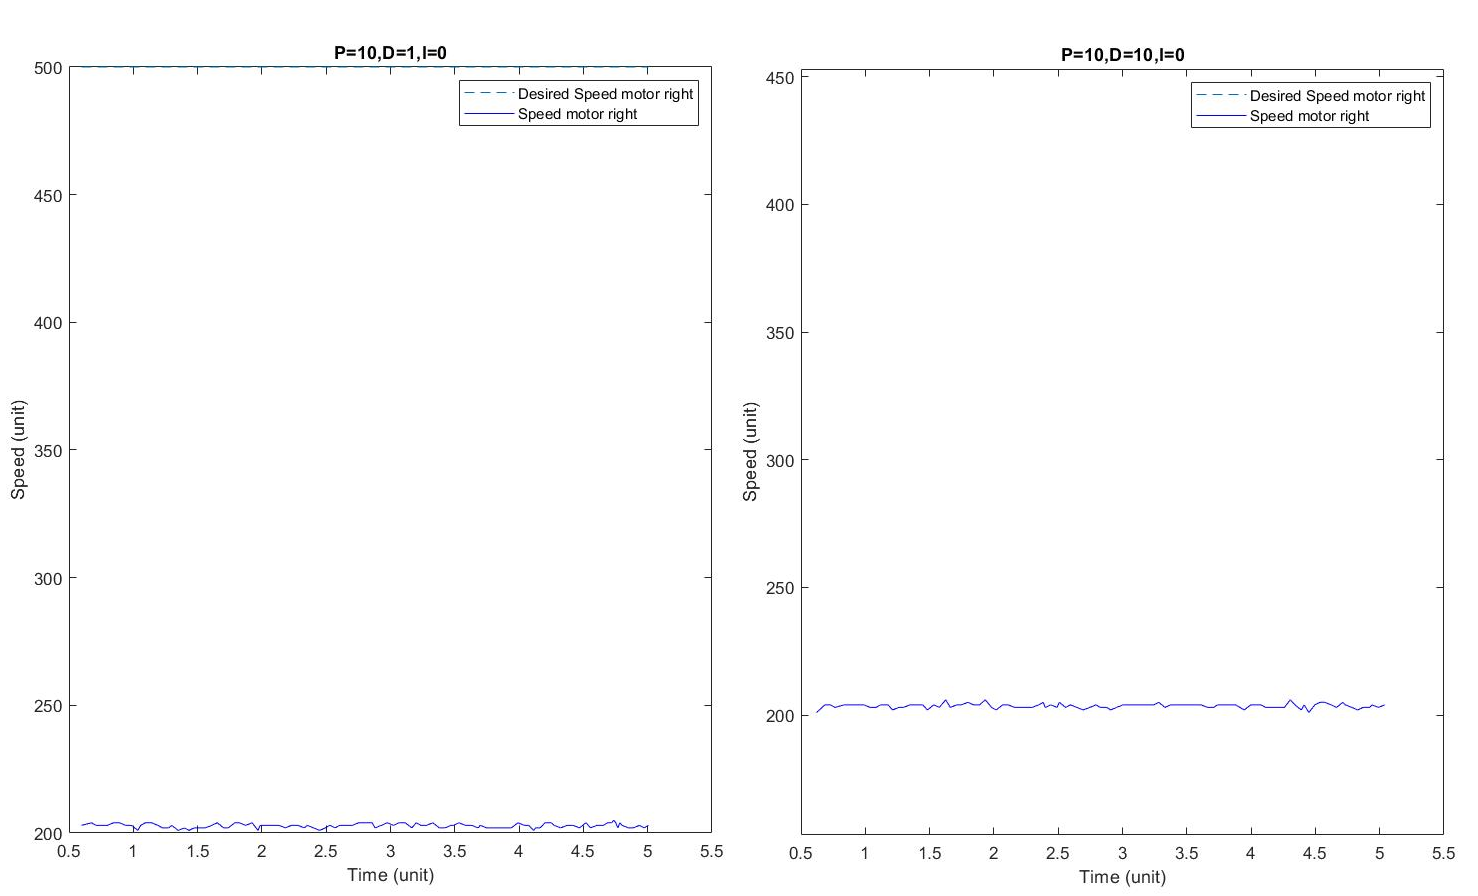
\includegraphics[width = 9cm]{imgs/fig7.png}
			\caption{}
		\end{figure}
		Nous réglons maintenant à P=10 D=10 et I = 1. Le temps de réponse est entre 1.3 et 1.4 s. Le système est moins rapide qu’avant mais il n’y a aucun dépassement et les variations de l’erreur sont plus faibles que précédemment. Nous allons garder ces paramètres et les étudier en leur infligeant des perturbations.\\

		\begin{figure}[h]
			\centering
			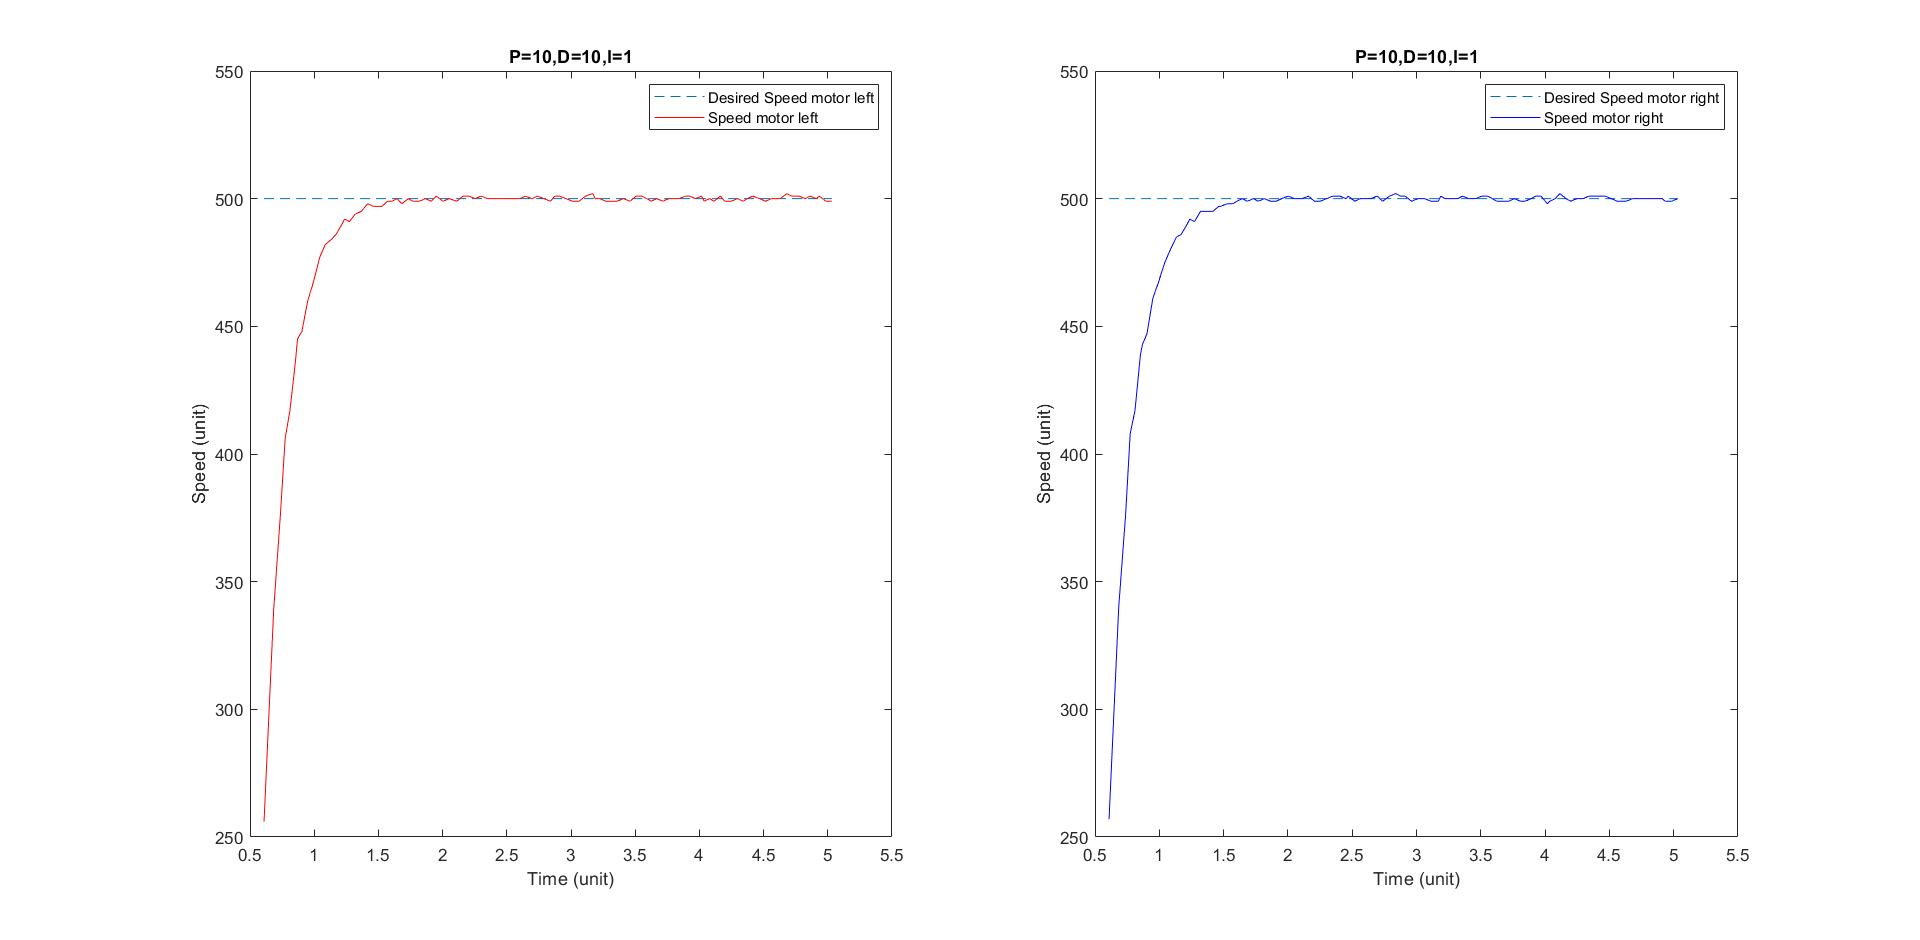
\includegraphics[width = 11cm]{imgs/fig8.jpg}
			\caption{}
		\end{figure}
		Nous voyons que le système redevient stable après la perturbation sur la roue droite mais le dépassement est trop important, il faudrait que la composante intégrale soit plus importante.
		
		\begin{figure}[h]
			\centering
			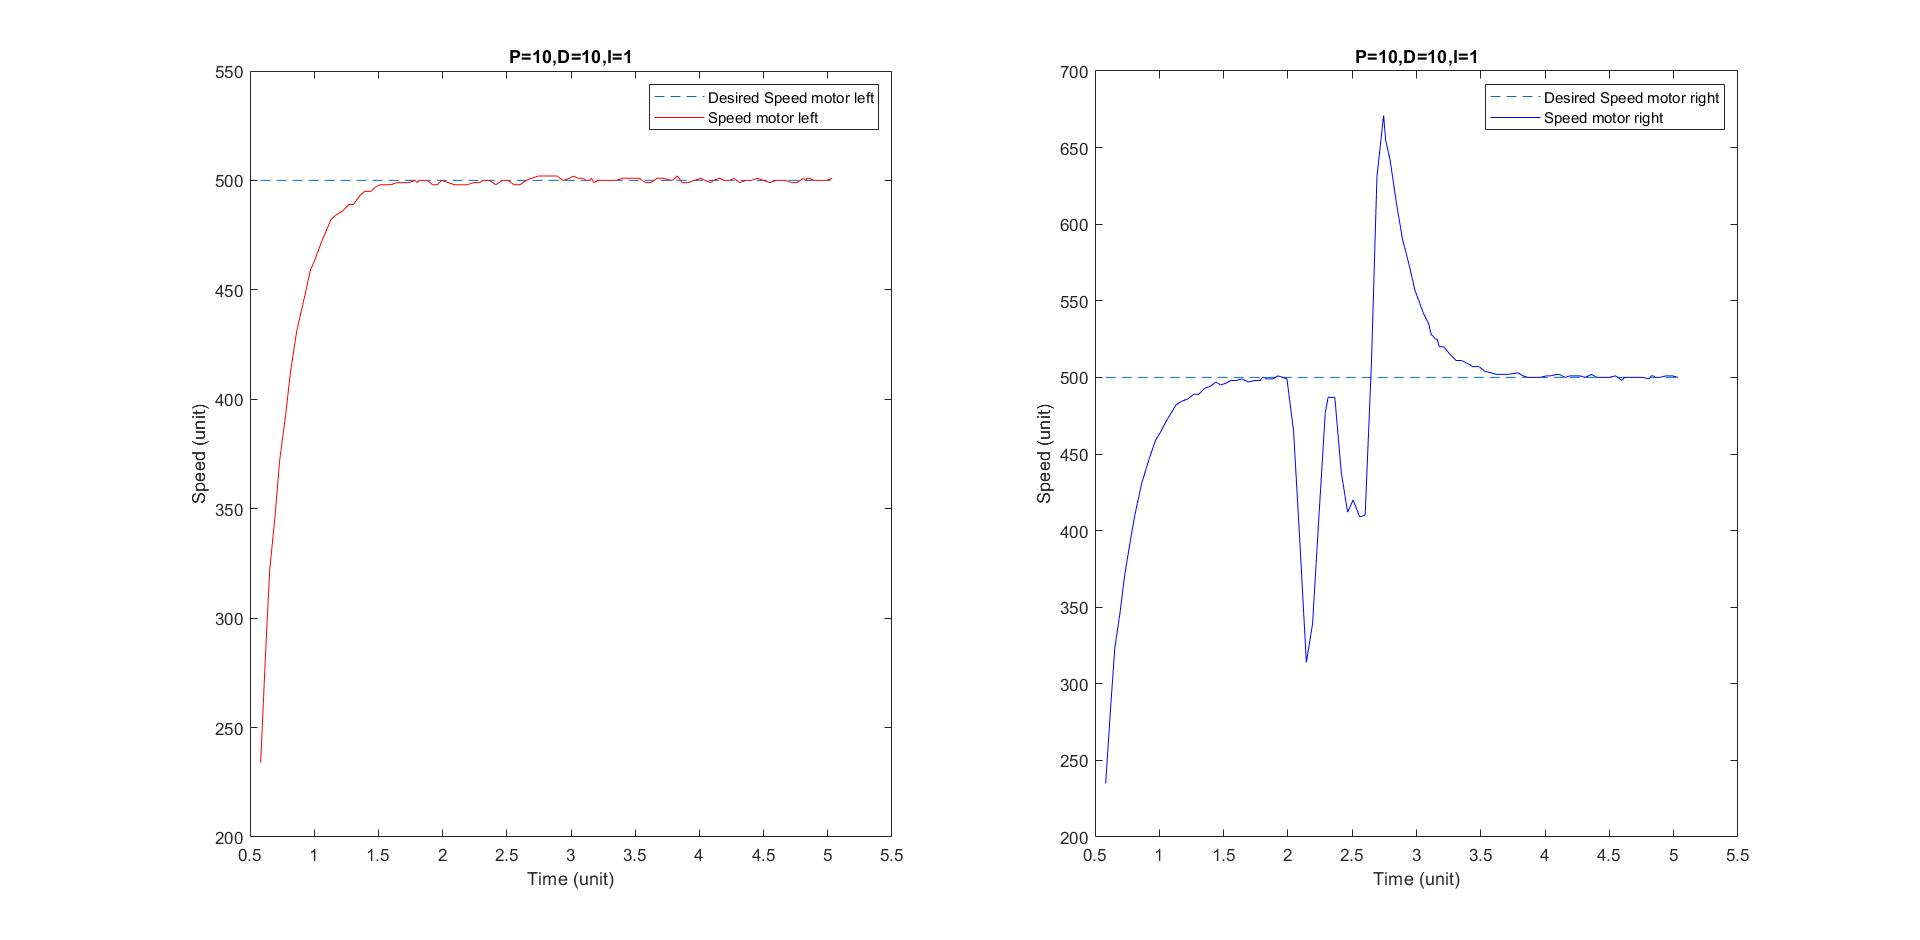
\includegraphics[width = 11cm]{imgs/fig9.jpg}
			\caption{}
		\end{figure}
		Nous allons aussi essayer de guider notre robot en changeant les valeurs des consignes. Nous avons choisi de commander le robot pour qu’il aille tout droit s’arrête puis tourne à droite.
		\newpage
		
		\begin{figure}[h]
			\centering
			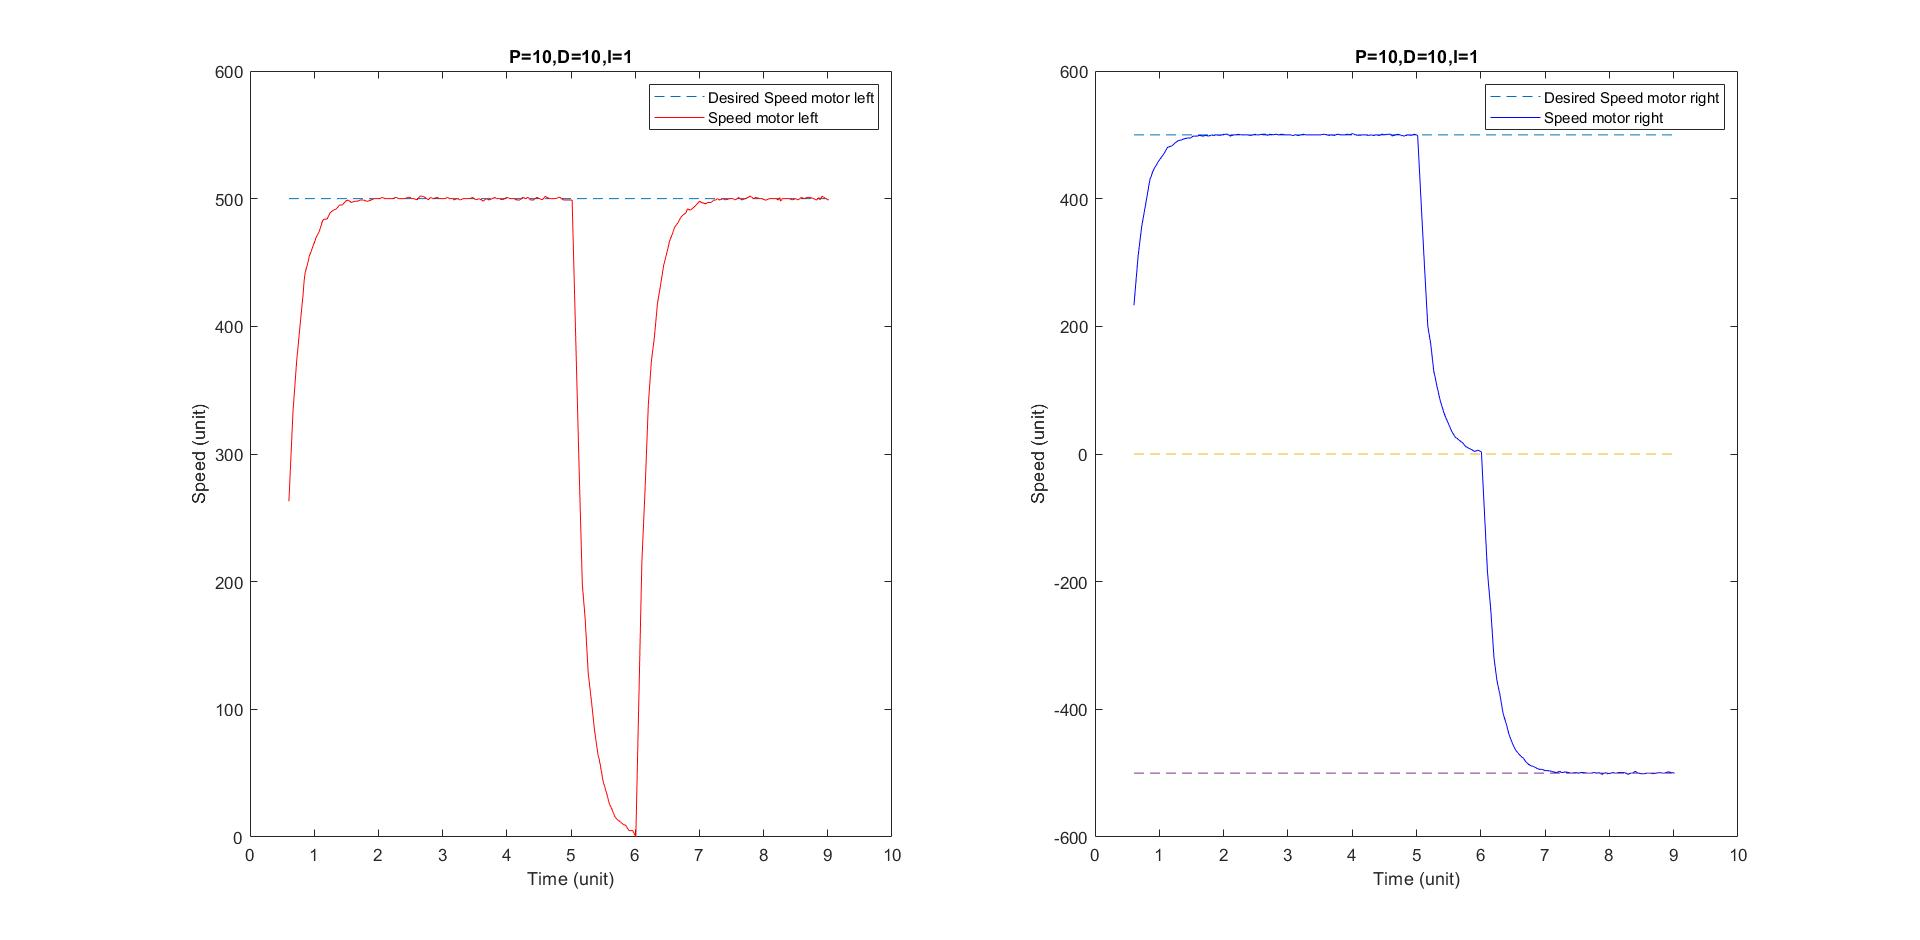
\includegraphics[width = 11cm]{imgs/fig10.jpg}
			\caption{}
		\end{figure}
		Avec les résultats observés nous voyons que pour différentes valeurs de consignes le système du robot est bien stable. 
		Ainsi nous avons étudié deux différentes commandes, la vitesse et la position. 
		La position permet de se rendre d’un point A à un point B sans prendre en compte la trajectoire suivie.
		La commande en vitesse permet de gérer la trajectoire du robot mais ils se déplacent indéfiniment dans l’espace. Nous pouvons contrôler la trajectoire du robot en changeant la consigne. 
		En ce qui concerne les performances, la commande en position est plus lente mais bien plus précise que la commande en vitesse. En effet, les deux commandes sont stables, il faut donc tirer profit de leurs avantages selon le contexte d’utilisation du robot. 
		
	
	\subsection{Clonclusion}
	P: Proportionnel, ce paramètre va gérer un gain brut. En général, plus il sera grand, plus il atteindra rapidement
	la valeur de la commande (voir trop rapidement et risque le plantage du robot ainsi que des dépassement de la commande)
	Il vas faire un gain constant à toutes les réactions du robot, il va surtout influer sur la rapidité.
		
	I: intégral, il va surtout influer sur la précision (de la commande vitesse ainsi que la commande position), il influe très peu sur la rapidité du système et un peu sur la stabilité. En effet, ce paramètre influe beaucoup sur la précision du système et nous permet de supprimer l'erreur constante si celle-ci est présente. Cette erreur constante est visible en zoomant sur les courbes, on remarque alors une erreur constante qu'il faut corriger.
	
	D: différentiel, il agit très peu sur la rapidité, un peu sur la précision mais influe énormément sur la stabilité. En effet, lors d'une perturbation, un changement brutal sera appliqué au système, donc une dérivée importante. C'est sur ce paramètre que l'on corrige le mieux ces perturbations.
	Attention, si il est trop fort, celui-ci risque juste de rendre le système instable.
	
	\begin{center}
		\begin{tabular}{||c|c|c|c||}
			\hline
			 & Rapidité & Stabilité & Précision \\[0.5ex]
			\hline \hline
			Kp & +++ & +++ & ++ \\
			\hline
			Kd & ++ & +++ & ++ \\
			\hline
			Ki & + & + & +++\\
			\hline
		\end{tabular}
	\end{center}

\end{document}